% !Mode:: "TeX:UTF-8"

\chapter{功能创新}

在第四阶段完成后,我们意识到该项目还有许多值得改进和优化的地方,于是打算添加一些新功能。

\section{会员功能}
\subsection{项目需求}
在首页,我们发现有一个注册会员入口,而这个功能在课程中并未实现,于是我们首先选择添加一个会员功能。
用户可以选择注册成为不同等级的会员从而享受到不同程度的折扣。
用户在支付订单页面可以查看打折后的价格,点击支付以支付优惠价。

\subsection{项目设计}
用户在首页可以点击“立即开通”可以进入会员注册界面,
有三种会员可以选择,分别是白银会员、黄金会员和钻石会员。
每种会员的价格不同,折扣力度也不同。
点击“去注册”可以发送注册请求。
注册请求分为3种情况:

1.如果用户不是会员,则会注册为选择的会员;

2.如果用户已经是会员且选择的会员比原本的会员等级高,则会升级会员;

3.如果用户已经是会员但选择的会员等级低于原本的会员等级,则会注册失败并返回错误信息。

\subsubsection*{接口文档}
Membership

1.MembershipController/getMembershipById(post方法)

参数:user

返回值:grade会员等级

功能:查询当前用户的会员等级

2.MembershipController/saveMembership(post方法)

参数:userId、grade

返回值:数据库改变的行数

功能:为一个用户注册会员

3.MembershipController/updateMembership(post方法)

参数:userId、grade

返回值:数据库改变的行数

功能:为一个用户升级会员

\subsection{实现结果}
\begin{figure}[H]
    \centering
    \subfigure{
        \begin{minipage}[t]{0.48\linewidth}
            \centering
            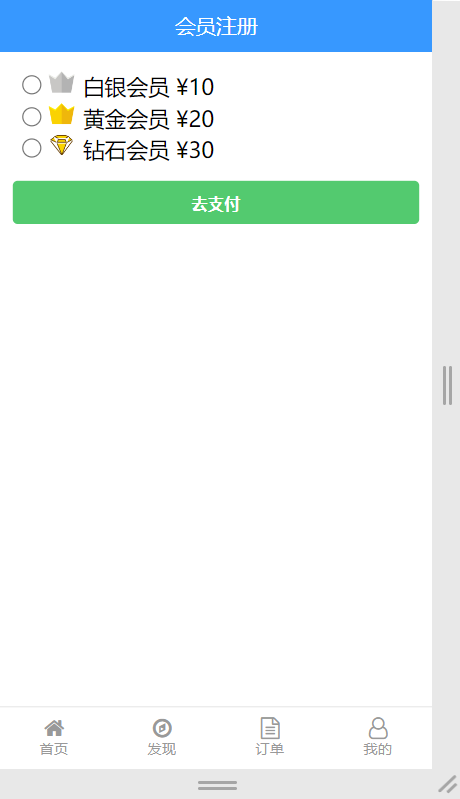
\includegraphics[scale=0.5]{figures/5.1.1.png}\\
        \end{minipage}
    }
    \subfigure{
        \begin{minipage}[t]{0.48\linewidth}
            \centering
            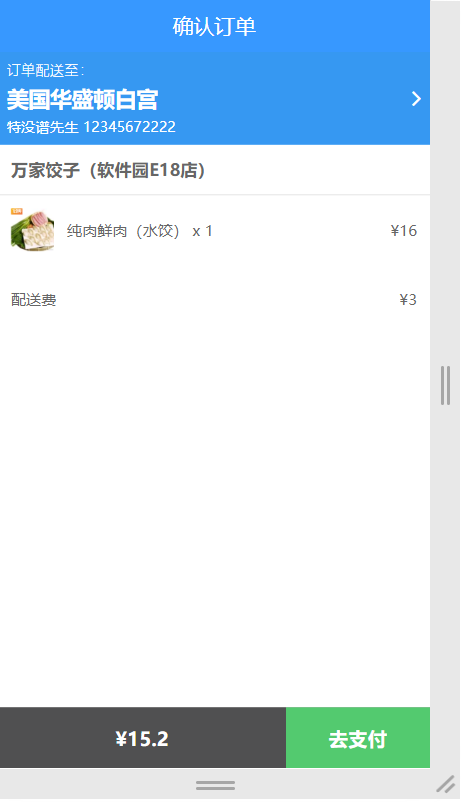
\includegraphics[scale=0.5]{figures/5.1.2.png}\\
        \end{minipage}
    }
    \centering
    \caption{会员功能实现结果}
\end{figure}

\section{“我的”页面}
\subsection{项目需求}
在网页下方的导航栏有一个“我的”按钮,在原来的实现中点击这个按钮并不会跳转到任何页面,于是我们决定实现一个“我的”页面。

\subsection{项目设计}
“我的”页面最上面会显示用户姓名、ID和会员等级,若未注册会员则默认为普通会员。
在用户信息的下面,添加“我的地址”和“注册会员”按钮,分别可以路由到编辑地址和注册会员页面。

\subsection*{接口文档}
MyProfile

1.MembershipController/getMembershipById(post方法)

参数:user

返回值:grade会员等级

功能:查询当前用户的会员等级

\subsection{实现结果}
\begin{figure}[H]
    \centering
    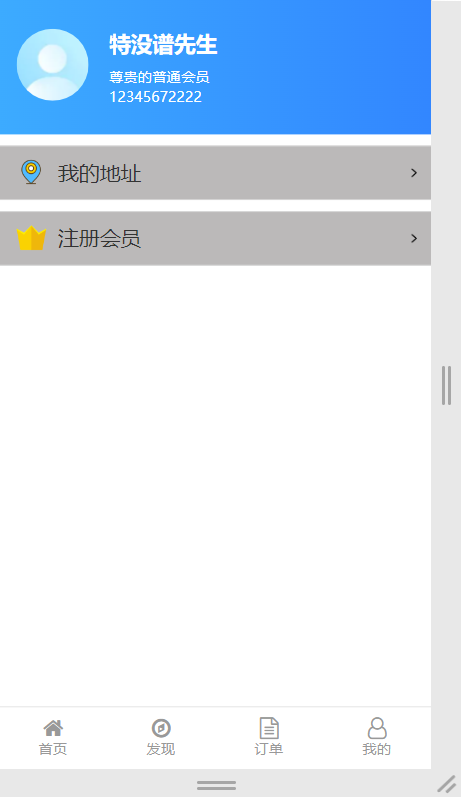
\includegraphics[scale=0.5]{figures/5.1.3.png}
    \caption{“我的”页面实现结果}
\end{figure}

\section{评论功能}
\subsection{项目需求}
在日常使用外卖APP时,我们经常会查看用户对商家的评价,
于是我们打算实现一个商家评论功能方便用户查看一个商家的评价

\subsection{项目设计}
用户在支付了一个订单之后,在订单页面可以点击“去评价”,用户进入评价页面可以编写评价,点击发布即可成功发布。
点击商家信息界面中的“评价”按钮可以进入商家评价页面查看自己和其他人的评价,每条评价会显示评价人姓名、会员等级、评价时间和评价内容。

\subsection*{接口文档}
Comment

1.CommentController/listCommentByBusinessId

参数:businessId

返回值:commentArr

功能:得到评论数据库的所有内容

2.CommentController/saveComment

参数:userId、userName、businessId、content、grade

返回值:数据库改变的行数

功能:保存一个评论

\subsection{实现结果}
\begin{figure}[H]
    \centering
    \subfigure{
        \begin{minipage}[t]{0.48\linewidth}
            \centering
            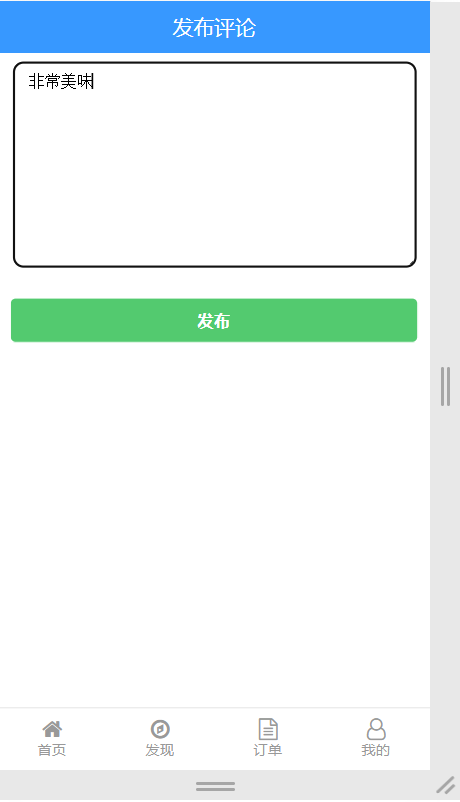
\includegraphics[scale=0.5]{figures/5.1.4.png}\\
        \end{minipage}
    }
    \subfigure{
        \begin{minipage}[t]{0.48\linewidth}
            \centering
            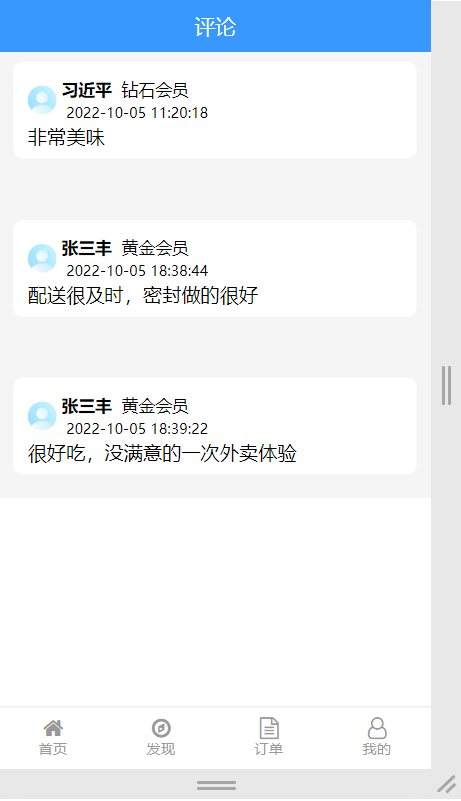
\includegraphics[scale=0.5]{figures/5.1.5.png}\\
        \end{minipage}
    }
    \centering
    \caption{评论员功能实现结果}
\end{figure}



